\chapter{Loops and strings}

Computers are often used to automate repetitive tasks.
Repeating tasks without making errors is something that computers do well and people do poorly.

\index{iteration}

Running the same code multiple times is called {\bf iteration}.
We have seen methods, like \java{countdown} and \java{factorial}, that use recursion to iterate.
Although recursion is elegant and powerful, it takes some getting used to.
Java provides language features that make iteration much easier:
the \java{while} and \java{for} statements.


\section{Assignment revisited}

TODO: ++, --, +=, -=


\section{The while statement}
\label{while}

\index{while}
\index{loop!while}
\index{statement!while}

Using a \java{while} statement, we can rewrite \java{countdown} like this:

\begin{code}
public static void countdown(int n) {
    while (n > 0) {
        System.out.println(n);
        n = n - 1;
    }
    System.out.println("Blastoff!");
}
\end{code}

You can almost read the \java{while} statement like English:
``While \java{n} is greater than zero, print the value of \java{n} and then reduce the value of \java{n} by 1.
When you get to zero, print Blastoff!''

\index{loop body}

The expression in parentheses is called the condition.
The statements in braces are called the {\bf body}.
The flow of execution for a \java{while} statement is:

\begin{enumerate}

\item Evaluate the condition, yielding \java{true} or \java{false}.

\item If the condition is \java{false}, skip the body and go to the next statement.

\item If the condition is \java{true}, execute the body and go back to step 1.

\end{enumerate}

\index{loop}

This type of flow is called a {\bf loop}, because the last step loops back around to the first.

\index{infinite loop}
\index{loop!infinite}

The body of the loop should change the value of one or more variables so that, eventually, the condition becomes \java{false} and the loop terminates.
Otherwise the loop will repeat forever, which is called an {\bf infinite loop}.
An endless source of amusement for computer scientists is the observation that the directions on shampoo, ``Lather, rinse, repeat,'' are an infinite loop.

In the case of \java{countdown}, we can prove that the loop terminates when \java{n} is positive.
But in general, it is not so easy to tell whether a loop terminates.
For example, this loop continues until \java{n} is 1 (which makes the condition \java{false}):

\begin{code}
public static void sequence(int n) {
    while (n != 1) {
        System.out.println(n);
        if (n % 2 == 0) {         // n is even
            n = n / 2;
        } else {                  // n is odd
            n = n * 3 + 1;
        }
    }
}
\end{code}

Each time through the loop, the program displays the value of \java{n} and then checks whether it is even or odd.
If it is even, the value of \java{n} is divided by two.
If it is odd, the value is replaced by $3n+1$.
For example, if the starting value (the argument passed to \java{sequence}) is 3, the resulting sequence is 3, 10, 5, 16, 8, 4, 2, 1.

Since \java{n} sometimes increases and sometimes decreases, there is no obvious proof that \java{n} will ever reach 1 and that the program will ever terminate.
For some values of \java{n}, we can prove that it terminates.
For example, if the starting value is a power of two, then the value of \java{n} will be even every time through the loop until we get to 1.
The previous example ends with such a sequence, starting when \java{n} is 16.

The hard question is whether this program terminates for {\em all} values of n.
So far, no one has been able to prove it {\em or} disprove it!
For more information, see \url{https://en.wikipedia.org/wiki/Collatz_conjecture}.
%The field of computer science is interested in these types of questions, because their answers give insight to the limits of what computers can and cannot do.


\section{The for statement}
\label{for}

\index{for}
\index{loop!for}
\index{statement!for}

The loops we have written so far have several elements in common.
They start by initializing a variable, they have a condition that depends on that variable, and inside the loop they do something to update that variable.
This type of loop is so common that there is another statement, the \java{for} loop, that expresses it more concisely.

For example, we could rewrite \java{printTable} like this:

\begin{code}
public static void printTable(int rows) {
    for (int i = 1; i <= rows; i = i + 1) {
        printRow(i, rows);
    }
}
\end{code}

\java{for} loops have three components in parentheses, separated by semicolons: the initializer, the condition, and the update.

\begin{enumerate}

\item The {\em initializer} runs once at the very beginning of the loop.

\item The {\em condition} is checked each time through the loop.
If it is \java{false}, the loop ends.
Otherwise, the body of the loop is executed (again).

\item At the end of each iteration, the {\em update} runs, and we go back to step 2.

\end{enumerate}

The \java{for} loop is often easier to read because it puts all the loop-related statements at the top of the loop.

There is one difference between \java{for} loops and \java{while} loops: if you declare a variable in the initializer, it only exists inside the \java{for} loop.
For example, here is a version of \java{printRow} that uses a \java{for} loop:

\begin{code}
public static void printRow(int n, int cols) {
    for (int i = 1; i <= cols; i = i + 1) {
        System.out.printf("%4d", n * i);
    }
    System.out.println(i);  // compiler error
}
\end{code}

The last line tries to display \java{i} (for no reason other than demonstration) but it won't work.
If you need to use a loop variable outside the loop, you have to declare it outside the loop, like this:

\begin{code}
public static void printRow(int n, int cols) {
    int i;
    for (i = 1; i <= cols; i = i + 1) {
        System.out.printf("%4d", n * i);
    }
    System.out.println(i);
}
\end{code}

\index{increment}
\index{decrement}

Assignments like \java{i = i + 1} don't often appear in \java{for} loops, because Java provides a more concise way to add and subtract by one.
Specifically, \java{++} is the {\bf increment} operator; it has the same effect as \java{i = i + 1}.
And \java{--} is the {\bf decrement} operator; it has the same effect as \java{i = i - 1}.

If you want to increment or decrement a variable by an amount other than \java{1}, you can use \java{+=} and \java{-=}.
For example, \java{i += 2} increments \java{i} by \java{2}.


\section{Characters}

\index{charAt}
\index{char}
\index{type!char}

Strings provide a method named \java{charAt}, which extracts a character.
It returns a \java{char}, a primitive type that stores an individual character (as opposed to strings of them).

\begin{code}
String fruit = "banana";
char letter = fruit.charAt(0);
\end{code}

The argument \java{0} means that we want the letter at position 0.
Like array indexes, string indexes start at 0, so the character assigned to \java{letter} is \java{b}.

Characters work like the other primitive types we have seen.
You can compare them using relational operators:

\begin{code}
if (letter == 'a') {
    System.out.println('?');
}
\end{code}

\index{quote mark}
\index{escape sequence}

Character literals, like \java{'a'}, appear in single quotes.
Unlike string literals, which appear in double quotes, character literals can only contain a single character.
Escape sequences, like \java{'\\t'}, are legal because they represent a single character.

The increment and decrement operators work with characters.
So this loop displays the letters of the alphabet:

\begin{code}
System.out.print("Roman alphabet: ");
for (char c = 'A'; c <= 'Z'; c++) {
    System.out.print(c);
}
System.out.println();
\end{code}

\index{Unicode}

Java uses {\bf Unicode} to represent characters, so strings can store text in other alphabets like Cyrillic and Greek, and non-alphabetic languages like Chinese.
You can read more about it at \url{http://unicode.org/}.

In Unicode, each character is represented by a ``code point'', which you can think of as an integer.
The code points for uppercase Greek letters run from 913 to 937, so we can display the Greek alphabet like this:

\begin{code}
System.out.print("Greek alphabet: ");
for (int i = 913; i <= 937; i++) {
    System.out.print((char) i);
}
System.out.println();
\end{code}

This example uses a type cast to convert each integer (in the range) to the corresponding character.


\section{String traversal}
\label{stringtraverse}

\index{traverse}

The following loop traverses the characters in \java{fruit} and displays them, one on each line:

\begin{code}
for (int i = 0; i < fruit.length(); i++) {
    char letter = fruit.charAt(i);
    System.out.println(letter);
}
\end{code}

\index{string!length}
\index{length!string}

Strings provide a method called \java{length} that returns the number of characters in the string.
Because it is a method, you have to invoke it with the empty argument list, \java{()}.
%Do not confuse \java{string.length()}, which is a method, with \java{array.length}, which is a constant.

\index{loop variable}
\index{variable!loop}

The condition is \java{i < fruit.length()}, which means that when \java{i} is equal to the length of the string, the condition is \java{false} and the loop terminates.

\index{toCharArray}

Unfortunately, the enhanced \java{for} loop does not work with strings.
But you can convert any string to a character array and iterate that:

\begin{code}
for (char letter : fruit.toCharArray()) {
    System.out.println(letter);
}
\end{code}

To find the last letter of a string, you might be tempted to try something like:

\begin{code}
int length = fruit.length();
char last = fruit.charAt(length);      // wrong!
\end{code}

\index{StringIndexOutOfBoundsException}
\index{exception!StringIndexOutOfBounds}

This code compiles and runs, but invoking the \java{charAt} method throws a \java{StringIndexOutOfBoundsException}.
The problem is that there is no sixth letter in \java{"banana"}.
Since we started counting at 0, the 6 letters are indexed from 0 to 5.
To get the last character, you have to subtract 1 from \java{length}.

\begin{code}
int length = fruit.length();
char last = fruit.charAt(length - 1);  // correct
\end{code}

Many string traversals involve reading one string and creating another.
For example, to reverse a string, we simply add one character at a time:

\begin{code}
public static String reverse(String s) {
    String r = "";
    for (int i = s.length() - 1; i >= 0; i--) {
        r = r + s.charAt(i);
    }
    return r;
}
\end{code}

\index{empty string}

The initial value of \java{r} is \java{""}, which is the {\bf empty string}.
The loop traverses the letters of \java{s} in reverse order.
Each time through the loop, it creates a new string and assigns it to \java{r}.
When the loop exits, \java{r} contains the letters from \java{s} in reverse order.
So the result of \java{reverse("banana")} is \java{"ananab"}.


\section{Substrings}

The \java{substring} method returns a new string that copies letters from an existing string, starting at the given index.

\begin{itemize}
\item \java{fruit.substring(0)} returns \java{"banana"}
\item \java{fruit.substring(2)} returns \java{"nana"}
\item \java{fruit.substring(6)} returns \java{""}
\end{itemize}

The first example returns a copy of the entire string.
The second example returns all but the first two characters.
As the last example shows, \java{substring} returns the empty string if the argument is the length of the string.

To visualize how the \java{substring} method works, it helps to draw a picture like Figure~\ref{fig.banana}.

\begin{figure}[!ht]
\begin{center}
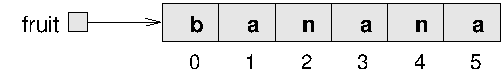
\includegraphics{figs/banana.pdf}
\caption{Memory diagram for a \java{String} of six characters.}
\label{fig.banana}
\end{center}
\end{figure}

%\begin{center}
%\begin{tabular}{c|c|c|c|c|c}
%%\hline
%b & a & n & a & n & a \\
%\hline
%0 & 1 & 2 & 3 & 4 & 5 \\
%%\hline
%\end{tabular}
%\end{center}

Like most string methods, \java{substring} is overloaded.
That is, there are other versions of \java{substring} that have different parameters.
If it's invoked with two arguments, they are treated as a start and end index:

\begin{itemize}
\item \java{fruit.substring(0, 3)} returns \java{"ban"}
\item \java{fruit.substring(2, 5)} returns \java{"nan"}
\item \java{fruit.substring(6, 6)} returns \java{""}
\end{itemize}

Notice that the character indicated by the end index is not included.
Defining \java{substring} this way simplifies some common operations.
For example, to select a substring with length \java{len}, starting at index \java{i}, you could write \java{fruit.substring(i, i + len)}.


\section{The indexOf method}

\index{indexOf}

The \java{indexOf} method searches for a character in a string.

\begin{code}
String fruit = "banana";
int index = fruit.indexOf('a');
\end{code}

This example finds the index of \java{'a'} in the string.
But the letter appears three times, so it's not obvious what \java{indexOf} should do.
According to the documentation, it returns the index of the {\em first} appearance.

To find subsequent appearances, you can use another version of \java{indexOf}, which takes a second argument that indicates where in the string to start looking.

\begin{code}
int index = fruit.indexOf('a', 2);
\end{code}

This code starts at index 2 (the first \java{'n'}) and finds the next \java{'a'}, which is at index 3.
If the letter happens to appear at the starting index, the starting index is the answer.
So \java{fruit.indexOf('a', 5)} returns \java{5}.

If the character does not appear in the string, \java{indexOf} returns \java{-1}.
Since indexes cannot be negative, this value indicates the character was not found.

You can also use \java{indexOf} to search for a substring, not just a single character.
For example, the expression \java{fruit.indexOf("nan")} returns \java{2}.


\section{String comparison}
\label{strcmp}

\index{equals}
\index{compareTo}

To compare two strings, it may be tempting to use the \java{==} and \java{!=} operators.

\begin{code}
String name1 = "Alan Turing";
String name2 = "Ada Lovelace";
if (name1 == name2) {                 // wrong!
    System.out.println("The names are the same.");
}
\end{code}

This code compiles and runs, and most of the time it gets the answer right.
But it is not correct, and sometimes it gets the answer wrong.
The problem is that the \java{==} operator checks whether the two variables refer to the same object (by comparing the references).
If you give it two different strings that contain the same letters, it yields \java{false}.

The right way to compare strings is with the \java{equals} method, like this:

\begin{code}
if (name1.equals(name2)) {
    System.out.println("The names are the same.");
}
\end{code}

This example invokes \java{equals} on \java{name1} and passes \java{name2} as an argument.
The \java{equals} method returns \java{true} if the strings contain the same characters; otherwise it returns \java{false}.

If the strings differ, we can use \java{compareTo} to see which comes first in alphabetical order:

\begin{code}
int diff = name1.compareTo(name2);
if (diff == 0) {
    System.out.println("The names are the same.");
} else if (diff < 0) {
    System.out.println("name1 comes before name2.");
} else if (diff > 0) {
    System.out.println("name2 comes before name1.");
}
\end{code}

The return value from \java{compareTo} is the difference between the first characters in the strings that differ.
If the strings are equal, their difference is zero.
If the first string (the one on which the method is invoked) comes first in the alphabet, the difference is negative.
Otherwise, the difference is positive.

In the preceding code, \java{compareTo} returns positive 8, because the second letter of \java{"Ada"} comes before the second letter of \java{"Alan"} by 8 letters.

\index{case-sensitive}

Both \java{equals} and \java{compareTo} are case-sensitive.
The uppercase letters come before the lowercase letters, so \java{"Ada"} comes before \java{"ada"}.


\section{String formatting}

\index{printf}
\index{utility method}

In Section~\ref{printf}, we learned how to use \java{printf} to display formatted output.
Sometimes programs need to create strings that are formatted a certain way, but not display them immediately, or ever.
For example, the following method returns a time string in 12-hour format:

\begin{code}
public static String timeString(int hour, int minute) {
    String ampm;
    if (hour < 12) {
        ampm = "AM";
        if (hour == 0) {
            hour = 12;  // midnight
        }
    } else {
        ampm = "PM";
        hour = hour - 12;
    }
    return String.format("%02d:%02d %s", hour, minute, ampm);
}
\end{code}

\index{string!format}

\java{String.format} takes the same arguments as \java{System.out.printf}: a format specifier followed by a sequence of values.
The main difference is that \java{System.out.printf} displays the result on the screen; \java{String.format} creates a new string, but does not display anything.

In this example, the format specifier \java{\%02d} means ``two digit integer padded with zeros'', so \java{timeString(19, 5)} returns the string \java{"07:05 PM"}.


\section{Nested Loops}

TODO


\section{Vocabulary}

\begin{description}

\term{iteration}
Executing a sequence of statements repeatedly.

\term{loop}
A statement that executes a sequence of statements repeatedly.

\term{loop body}
The statements inside the loop.

\term{infinite loop}
A loop whose condition is always true.

\term{program development}
A process for writing programs.
So far we have seen ``incremental development'' and ``encapsulation and generalization''.

\term{encapsulate}
To wrap a sequence of statements in a method.

\term{generalize}
To replace something unnecessarily specific (like a constant value) with something appropriately general (like a variable or parameter).

\term{loop variable}
A variable that is initialized, tested, and updated in order to control a loop.

\term{increment}
Increase the value of a variable.

\term{decrement}
Decrease the value of a variable.

\term{pretest loop}
A loop that tests the condition before each iteration.

\term{posttest loop}
A loop that tests the condition after each iteration.

\end{description}


\section{Exercises}

The code for this chapter is in the {\tt ch06} directory of {\tt ThinkJavaCode2}.
See page~\pageref{code} for instructions on how to download the repository.
Before you start the exercises, we recommend that you compile and run the examples.

If you have not already read Appendix~\ref{debugger}, now might be a good time.
It describes the DrJava debugger, which is a useful tool for visualizing the flow of execution through loops.


\begin{exercise}  %%V6 Ex7.1

Consider the following methods:

\begin{code}
public static void main(String[] args) {
    loop(10);
}

public static void loop(int n) {
    int i = n;
    while (i > 1) {
        System.out.println(i);
        if (i % 2 == 0) {
            i = i / 2;
        } else {
            i = i + 1;
        }
    }
}
\end{code}

\begin{enumerate}

\item Draw a table that shows the value of the variables \java{i} and \java{n} during the execution of \java{loop}.
The table should contain one column for each variable and one line for each iteration.

\item What is the output of this program?

\item Can you prove that this loop terminates for any positive value of \java{n}?

% If i is odd and we increment by 1, the result is even.  So the second
% branch is always followed by the first branch.
% If i is even and we divide by 2, the result might be odd.  So in the
% worst case, we might alternate between the branches.
% But we can't do more of the second branch than the first.
% So we divide at least as often as we add.

% If i is 1, we're done.
% If i is 2, we divide by 2 and we're done.
% If i is greater than 2, the first branch decreases more than the
% second branch increases.
% So if we do one of each, the net effect is a decrease.
% Therefore, the value of i has to decrease after any two steps.

\end{enumerate}

\end{exercise}


\begin{exercise}  %%V6 Ex7.2

Let's say you are given a number, $a$, and you want to find its square root.
One way to do that is to start with a rough guess about the answer, $x_0$, and then improve the guess using this formula:
%
\[ x_1 =(x_0 + a/x_0) / 2 \]
%
For example, if we want to find the square root of 9, and we start with $x_0 = 6$, then $x_1 = (6 + 9/6) / 2 = 3.75$, which is closer.
We can repeat the procedure, using $x_1$ to calculate $x_2$, and so on.
In this case, $x_2 = 3.075$ and $x_3 = 3.00091$.
So it converges quickly on the correct answer.

Write a method called \java{squareRoot} that takes a \java{double} and returns an approximation of the square root of the parameter, using this technique.
You should not use \java{Math.sqrt}.

As your initial guess, you should use $a/2$.
Your method should iterate until it gets two consecutive estimates that differ by less than 0.0001.
%In other words, return when the absolute value of $x_n - x_{n-1}$ is less than 0.0001.
You can use \java{Math.abs} to calculate the absolute value of the difference.

\end{exercise}


\begin{exercise}  %%V6 Ex7.3

In Exercise~\ref{ex.power} we wrote a recursive version of \java{power}, which takes a double \java{x} and an integer \java{n} and returns $x^n$.
Now write an iterative method to perform the same calculation.

\end{exercise}


\begin{exercise}  %%V6 Ex7.4

Section~\ref{factorial} presents a recursive method that computes the factorial function.
Write an iterative version of \java{factorial}.

\end{exercise}


\begin{exercise}  %%V6 Ex7.5

One way to calculate $e^x$ is to use the infinite series expansion:
%
\[ e^x = 1 + x + x^2 / 2! + x^3 / 3! + x^4 / 4! + \ldots \]
%
The $i$th term in the series is $x^i / i!$.

\begin{enumerate}

\item Write a method called \java{myexp} that takes \java{x} and \java{n} as parameters and estimates $e^x$ by adding the first \java{n} terms of this series.
You can use the \java{factorial} method from Section~\ref{factorial} or your iterative version from the previous exercise.

\index{efficiency}

\item You can make this method more efficient if you realize that the numerator of each term is the same as its predecessor multiplied by \java{x}, and the denominator is the same as its predecessor multiplied by \java{i}.
Use this observation to eliminate the use of \java{Math.pow} and \java{factorial}, and check that you get the same result.

\item Write a method called \java{check} that takes a parameter, \java{x}, and displays \java{x}, \java{myexp(x)}, and \java{Math.exp(x)}.
The output should look something like:

\begin{stdout}
1.0     2.708333333333333     2.718281828459045
\end{stdout}

You can use the escape sequence \java{"\\t"} to put a tab character between columns of a table.

\item Vary the number of terms in the series (the second argument that \java{check} sends to \java{myexp}) and see the effect on the accuracy of the result.
Adjust this value until the estimated value agrees with the correct answer when \java{x} is 1.

\item Write a loop in \java{main} that invokes \java{check} with the values 0.1, 1.0, 10.0, and 100.0.
How does the accuracy of the result vary as \java{x} varies?
Compare the number of digits of agreement rather than the difference between the actual and estimated values.

\item Add a loop in \java{main} that checks \java{myexp} with the values -0.1, -1.0, -10.0, and -100.0.
Comment on the accuracy.

\end{enumerate}

\end{exercise}


\begin{exercise}  %%V6 Ex7.6

One way to evaluate $\exp(-x^2)$ is to use the infinite series expansion:
%
\[ \exp(-x^2) = 1 - x^2 + x^4/2 - x^6/6 + \ldots \]
%
The $i$th term in this series is $(-1)^i x^{2i} / i!$.
Write a method named \java{gauss} that takes \java{x} and \java{n} as arguments and returns the sum of the first \java{n} terms of the series.
You should not use \java{factorial} or \java{pow}.

\end{exercise}
